\href{../README.md}{\textless--}

\begin{center}\rule{0.5\linewidth}{0.5pt}\end{center}

\section{Rappels \& compléments de C}\label{rappels-compluxe9ments-de-c}

\begin{itemize}
\tightlist
\item
  \hyperref[rappels--compluxe9ments-de-c]{Rappels \& compléments de C}

  \begin{itemize}
  \tightlist
  \item
    \hyperref[les-bases]{Les bases}

    \begin{itemize}
    \tightlist
    \item
      \hyperref[hello-world]{Hello world}
    \item
      \hyperref[pruxe9processeur]{Préprocesseur}
    \item
      \hyperref[types-de-variables]{Types de variables}
    \item
      \hyperref[tableaux]{Tableaux}
    \item
      \hyperref[caractuxe8res-ascii]{Caractères ASCII}
    \item
      \hyperref[les-pointeurs]{Les pointeurs}
    \item
      \hyperref[structures]{Structures}
    \item
      \hyperref[pointeur-vers-une-fonction]{Pointeur vers une fonction}
    \item
      \hyperref[expressions-de-manipulation-de-bits]{Expressions de
      manipulation de bits}
    \item
      \hyperref[constante]{Constante}
    \end{itemize}
  \end{itemize}
\end{itemize}

\subsection{Les bases}\label{les-bases}

\subsubsection{Hello world}\label{hello-world}

On se souvient que pour faire un programme en C il faut des choses
cruciales: 1. Directives préprocesseur
\texttt{\#include\ \textless{}stdio.h\textgreater{}} 2. Avoir une
fonction \texttt{main} qui est le point d'entrée de l'exécution 1.
Fournir les arguments \texttt{argc} et \texttt{argv{[}{]}} pour prendre
les arguments en ligne de commande. 3. Retourner un succès avec
\texttt{EXIT\_SUCCESS} 4. Compiler le programme avec \texttt{gcc} comme
cela \texttt{gcc\ -o\ output\ input.c}

\begin{Shaded}
\begin{Highlighting}[]
\PreprocessorTok{\#include }\ImportTok{\textless{}stdio.h\textgreater{}}
\PreprocessorTok{\#include }\ImportTok{\textless{}stdlib.h\textgreater{}}

\DataTypeTok{int}\NormalTok{ main}\OperatorTok{(}\DataTypeTok{int}\NormalTok{ argc}\OperatorTok{,} \DataTypeTok{char}\OperatorTok{*}\NormalTok{ argv}\OperatorTok{[])\{}
\NormalTok{    printf}\OperatorTok{(}\StringTok{"Hello world !}\SpecialCharTok{\textbackslash{}n}\StringTok{"}\OperatorTok{);}

    \ControlFlowTok{return}\NormalTok{ EXIT\_SUCCESS}\OperatorTok{;}
\OperatorTok{\}}
\end{Highlighting}
\end{Shaded}

\subsubsection{Préprocesseur}\label{pruxe9processeur}

Notre code C est transformé par ce préprocesseur avant d'être compilé en
langage machine.

C'est donc une traduction texte vers texte.

Pour obtenir le résultat du préprocesseur on fait \texttt{gcc\ -E}.

\paragraph{Include et header}\label{include-et-header}

Cela permet d'importer des fonctions, constantes d'un librairie.

\begin{itemize}
\tightlist
\item
  \textbf{Header}: contient les informations sur comment appeler une
  fonction et le squelette du code.
\item
  \textbf{Code source}: la mise en oeuvre des fonctions.
\end{itemize}

On fait \texttt{\#include\ "monheader.h"} pour inclure du dossier
courant et \texttt{\#include\ \textless{}header.h\textgreater{}} pour un
header standard. On peut avoir des infos sur un header via
\texttt{man\ 3\ stdio.h}.

\subsubsection{Types de variables}\label{types-de-variables}

Voir les slides car très basique

Il faut faire attention en C avec les notations des \texttt{int}: -
Notation classique: \texttt{i\ =\ 123} - Hexadécimal:
\texttt{i\ =\ 0x7b} - Octal: \texttt{i\ =\ 0173} - Binaire:
\texttt{i\ =\ 0b1111011}

La différence entre octal et classique est ce 0 au début.

On se souvient aussi des entiers \emph{unsigned} qui sont des entiers
qui ne peuvent être négatifs et donc pour le même nombre de bit peuvent
avoir un nombre plus élevé que leurs homologues \emph{signed}.

\subsubsection{Tableaux}\label{tableaux}

On se souvient qu'en C, la taille d'un array doit être connu à l'avance
! (sinon on doit utiliser malloc sur le heap)

\subsubsection{Caractères ASCII}\label{caractuxe8res-ascii}

\begin{figure}
\centering
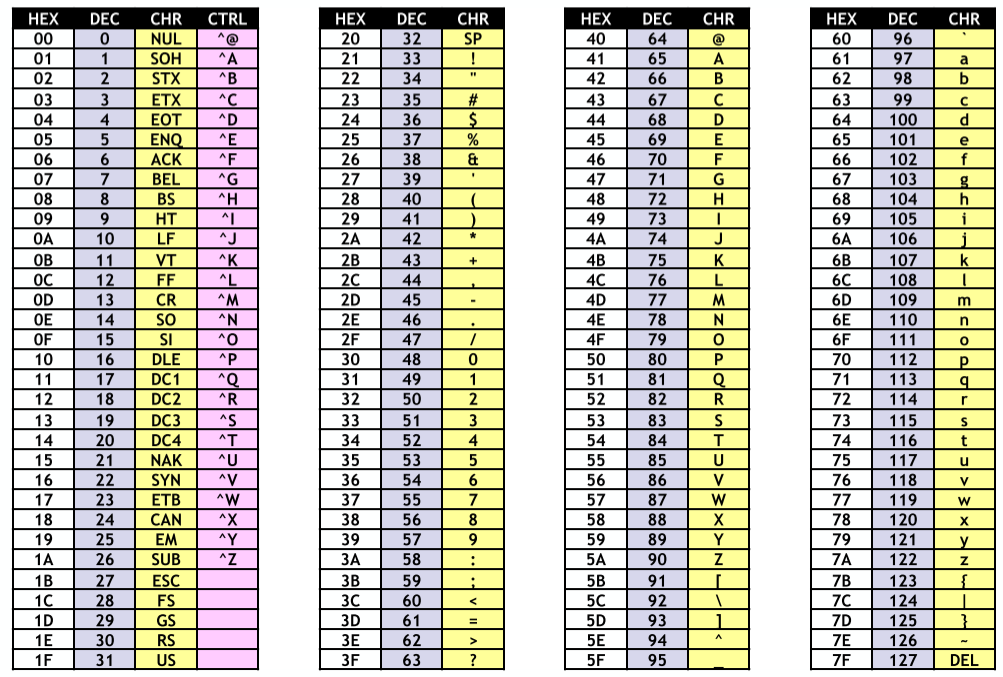
\includegraphics{image-6.png}
\caption{Alt text}
\end{figure}

\subsubsection{Les pointeurs}\label{les-pointeurs}

La mémoire est une sorte de ruban avec des cases (\emph{octets}) avec
des adresses consécutives. Les adresses sont des \textbf{entiers non
signés} de \textbf{32/64} bits selon le processeur ou jeu d'instruction.

Pour définir une variable d'un pointeur on fait:

\begin{Shaded}
\begin{Highlighting}[]
\DataTypeTok{int}\OperatorTok{*}\NormalTok{ ptr\_i}\OperatorTok{;} \CommentTok{// Défini un pointeur d\textquotesingle{}un int}
\OperatorTok{\&}\NormalTok{ptr\_i}\OperatorTok{;} \CommentTok{// Permet d\textquotesingle{}avoir l\textquotesingle{}adresse où est stocké ce pointeur}
\OperatorTok{*}\NormalTok{ptr\_i}\OperatorTok{;} \CommentTok{// Pour avoir la valeur pointée par le pointeur}
\end{Highlighting}
\end{Shaded}

On n'oublie pas qu'on peut faire des \textbf{opérations arithmétiques}
sur les pointeurs. (ex: aller à la case suivante, \ldots)

\begin{Shaded}
\begin{Highlighting}[]
\DataTypeTok{int}\NormalTok{ main}\OperatorTok{(}\DataTypeTok{int}\NormalTok{ argc}\OperatorTok{,} \DataTypeTok{char} \OperatorTok{**}\NormalTok{argv}\OperatorTok{)} \OperatorTok{\{} 
    
    \DataTypeTok{char} \OperatorTok{**}\NormalTok{p}\OperatorTok{;}\NormalTok{ p}\OperatorTok{=}\NormalTok{argv}\OperatorTok{;} 
\NormalTok{    printf}\OperatorTok{(}\StringTok{"Arguments :"}\OperatorTok{);} 
    \ControlFlowTok{while}\OperatorTok{(*}\NormalTok{p}\OperatorTok{!=}\NormalTok{NULL}\OperatorTok{)} \OperatorTok{\{} 
\NormalTok{        printf}\OperatorTok{(}\StringTok{" }\SpecialCharTok{\%s}\StringTok{"}\OperatorTok{,*}\NormalTok{p}\OperatorTok{);} 
\NormalTok{        p}\OperatorTok{++;}
    \OperatorTok{\}}
\NormalTok{    printf}\OperatorTok{(}\StringTok{"}\SpecialCharTok{\textbackslash{}n}\StringTok{"}\OperatorTok{);}
    \ControlFlowTok{return}\OperatorTok{(}\NormalTok{EXIT\_SUCCESS}\OperatorTok{);}
\OperatorTok{\}}
\end{Highlighting}
\end{Shaded}

Ici, on voit que à un moment donné, le pointeur sera \texttt{NULL} car
il n'y a plus de zone mémoire.

\subsubsection{Structures}\label{structures}

On n'a pas la notion d'objet en C mais on peut déclarer des types de
données personnalisées sous forme de structure.

\begin{Shaded}
\begin{Highlighting}[]
\KeywordTok{struct}\NormalTok{ coord}\OperatorTok{\{}
    \DataTypeTok{int}\NormalTok{ x}\OperatorTok{;}
    \DataTypeTok{int}\NormalTok{ y}\OperatorTok{;}
    \DataTypeTok{int}\NormalTok{ z}\OperatorTok{;}
\OperatorTok{\}}

\KeywordTok{struct}\NormalTok{ coord point }\OperatorTok{=} \OperatorTok{\{}\DecValTok{1}\OperatorTok{,} \DecValTok{2}\OperatorTok{,} \DecValTok{3}\OperatorTok{\};}
\NormalTok{point}\OperatorTok{.}\NormalTok{x}\OperatorTok{;}\NormalTok{ point}\OperatorTok{.}\NormalTok{y}\OperatorTok{;}\NormalTok{ point}\OperatorTok{.}\NormalTok{z}\OperatorTok{;}
\end{Highlighting}
\end{Shaded}

\paragraph{Alias}\label{alias}

Pour simplifier l'écriture de structure, on peut utiliser des
\textbf{alias}. On peut même renommer des types de données déjà existant
(ex: int, \ldots):

\begin{Shaded}
\begin{Highlighting}[]
\CommentTok{// structure pour stocker une fraction }
\KeywordTok{typedef} \KeywordTok{struct}\NormalTok{ fraction }\OperatorTok{\{} 
    \DataTypeTok{double}\NormalTok{ numerator}\OperatorTok{;} 
    \DataTypeTok{double}\NormalTok{ denominator}\OperatorTok{;} 
\OperatorTok{\}}\NormalTok{ Fraction }\OperatorTok{;}

\KeywordTok{typedef} \DataTypeTok{int}\NormalTok{ Entier}\OperatorTok{;}

\DataTypeTok{int}\NormalTok{ main}\OperatorTok{(}\DataTypeTok{int}\NormalTok{ argc}\OperatorTok{,} \DataTypeTok{char} \OperatorTok{*}\NormalTok{argv}\OperatorTok{[])} \OperatorTok{\{}
\NormalTok{    Fraction demi }\OperatorTok{=} \OperatorTok{\{}\DecValTok{1}\OperatorTok{,} \DecValTok{2}\OperatorTok{\};} 
\NormalTok{    Entier i }\OperatorTok{=} \DecValTok{2}\OperatorTok{;} 
    \CommentTok{// ... }
    \ControlFlowTok{return}\NormalTok{ EXIT\_SUCCESS}\OperatorTok{;}
\OperatorTok{\}}
\end{Highlighting}
\end{Shaded}

\paragraph{Tips}\label{tips}

Il existe un sucre syntaxique vraiment sympa:

\begin{Shaded}
\begin{Highlighting}[]
\OperatorTok{(*}\NormalTok{f}\OperatorTok{).}\NormalTok{value}\OperatorTok{;}
\NormalTok{f}\OperatorTok{{-}\textgreater{}}\NormalTok{value}\OperatorTok{;}
\end{Highlighting}
\end{Shaded}

Cela fait la même chose mais est plus simple (surtout avec les
parenthèses).

\subsubsection{Pointeur vers une
fonction}\label{pointeur-vers-une-fonction}

On peut stocker une fonction via son pointeur comme cela:

\begin{Shaded}
\begin{Highlighting}[]
\NormalTok{type\_retour }\OperatorTok{(*}\NormalTok{ptr\_vers\_func}\OperatorTok{)([}\NormalTok{type\_arg}\OperatorTok{]+);}
\DataTypeTok{void} \OperatorTok{(*}\NormalTok{f1}\OperatorTok{)(}\DataTypeTok{int}\OperatorTok{,} \DataTypeTok{int}\OperatorTok{,} \DataTypeTok{char}\OperatorTok{*);}
\DataTypeTok{int} \OperatorTok{(*}\NormalTok{f2}\OperatorTok{)(}\DataTypeTok{int}\OperatorTok{);}
\NormalTok{f2 }\OperatorTok{=} \OperatorTok{\&}\NormalTok{ma\_function}\OperatorTok{;}
\end{Highlighting}
\end{Shaded}

Ensuite pour faire un appel, on doit déréférencer le pointeur.

\subsubsection{Expressions de manipulation de
bits}\label{expressions-de-manipulation-de-bits}

\begin{longtable}[]{@{}cc@{}}
\toprule\noalign{}
Opération & Explication \\
\midrule\noalign{}
\endhead
\bottomrule\noalign{}
\endlastfoot
\texttt{\textasciitilde{}} & Inversion des bits \\
\texttt{\&} & Le ET \\
\texttt{\textbackslash{}\textbar{}} & le OU \\
\texttt{\^{}} & le XOR (seulement si 1 bit est 1) \\
\texttt{\textgreater{}\textgreater{}} & Shift les bits de x places vers
la droite \\
\end{longtable}

\subsubsection{Constante}\label{constante}

Pour définir une constante: - \textbf{Avant C99}:
\texttt{\#define\ M\_PI} puis mettre \texttt{3.14159;} - \textbf{Après
C99}: On utilise le mot-clé \texttt{const}.

Une variable globale est définie pour tous les modules d'un programme.

Une variable \texttt{static}, on peut y accéder en dehors d'un bloc de
fonction car on ne doit pas l'instancier.

\begin{center}\rule{0.5\linewidth}{0.5pt}\end{center}

\href{../README.md}{\textless--}
